\section{Alit Fajar Kurniawan}
{\Large \textbf{Pemahaman Teori}}
\subsection{No. 1}
Apa itu fungsi device manager di windows dan folder /dev di linux?

	\hfill \break
	Device manager adalah perangkat lunak untuk menampilkan seluruh perangkat keras yang diinisialisasi atau sudah terhubung dengan sistem operasi Windows. Perangkat keras tersebut bisa berupa harddisk, kartu VGA, sound, keyboard, perangkat USB dan lain-lainnya. fungsi lain dari device manager yaitu, Menunjukkan status mengenai suatu perangkat keras,
	Mengelola driver perangkat keras, Menonaktifkan dan mengaktifkan perangkat keras, Menunjukkan informasi detail mengenai suatu perangkat keras, Mengidentifikasi konflik antar perangkat keras, dan Memberitahukan terjadinya masalah pada perangkat keras.

	\hfill \break
	Folder /dev merupakan representasi dari drive yang terhubung ke sistem operasi Linux dan oleh sistem dianggap sebagai file-file direktori. Biasanya sering ditampilkan direktori seperti /dev/sda1 yang mewakili Drive SATA pertama dalam sistem.

\subsection{No. 2}
Jelaskan langkah-langkah instalasi driver dari arduino!

	\hfill \break
	Berikut ini adalah langkah-langkah instalasi driver dari Arduino UNO di Windows:

	\begin{enumerate}
		\item Pertama pastikan Arduino IDE telah terinstall.
		\item Lalu hubungkan port USB Arduino Uno ke port USB PC.
		\item Kemudian PC anda akan mendeteksi perangkat baru yang terpasang dan akan muncul pop seperti ini.
		\item Karena Arduino Uno baru pertama kali terpasang, maka akan muncul pop up error seperti ini.
		\item Buka ''Start'' lalu cari Device Manager, kemudian klik ''Device Manager''.
		\item Setelah Device Manager terbuka, silahkan cari ''Unknown Device'' yang berada di Other Device.
		\item Kemudian klik kanan pada ''Unknown Device'', lalu pilih ''Update Driver Software''.
		\item Setelah itu muncul window baru, lalu pilih ''Browse my computer for driver software''.
		\item Lalu cari folder yang terinstall Arduino IDE dengan mengklik browse. Kemudian klik ''Next''.
		\item Windows akan mencari dan menginstall driver yang berada pada folder tersebut.
		\item Setelah itu akan muncul window, lalu klik ''Install''.
		\item Jika berhasil terinstal maka akan muncul window seperti ini.
	\end{enumerate}

\subsection{No. 3}
	\begin{itemize}
		\item Membaca Baudrate dari Komputer
			\begin{enumerate}
				\item Pertama buka ''Start''. Cari ''Device Manager'', lalu klik.
				\item Kemudian pilih ''Ports (COM \& LPT)''.
				\item Klik dua kali pada COM yang terhubung.
				\item Pilih tab ''Port Settings'', lalu lihat di ''Bit per second''.
			\end{enumerate}
		\item Membaca Port dari Komputer
			\begin{enumerate}
				\item Pertama buka ''Start''. Cari ''Device Manager'', lalu klik.
				\item Kemudian pilih ''Ports (COM \& LPT)''.
				\item Port dari Arduino telah terbaca oleh PC.
			\end{enumerate}
	\end{itemize}
	
\subsection{No. 4}
	Jelaskan sejarah library pyserial!

	\hfill \break
	PySerial adalah paket Python yang menfasilitasi komunikasi serial antara PC dengan perangkat keras eksternal. PySerial menyediakan antarmuka untuk berkomunikasi melalui protokol komunikasi serial. Komunikasi serial adalah salah satu protokol komunikasi komputer tertua. Protokol komunikasi serial mendahului spesifikasi USB yang digunakan oleh komputer dan perangkat keras lain seperti mouse, keyboard, dan webcam. USB adalah singkatan dari Universal Serial Bus. USB dan dibangun di atas dan memperluas antarmuka komunikasi serial asli.

\subsection{No. 5}
	Jelaskan fungsi-fungsi apa saja yang dipakai dari library pyserial!

	\hfill \break
	Fungsi-fungsi yang dipakai dari library PySerial, yaitu:
	\begin{enumerate}
		\item Serial - fungsi ini untuk membuka port serial.
		\item write(data) - fungsi ini menulis data lewat port serial.
		\item readline - fungsi ini membaca sebuah string dari port serial.
		\item read(size) - fungsi ini untuk membaca jumlah byte dari port serial.
		\item close - fungsi ini untuk menutup port serial.
	\end{enumerate}

\subsection{No. 6}
	Jelaskan kenapa butuh perulangan dan tidak butuh perulangan dalam membaca serial!

	\hfill \break
	Pada saat membaca serial di Arduino diperlukan perulangan agar bisa membaca data secara berulang kali sehingga data yang muncul banyak. Sedangkan apabila tidak membutuhkan perulangan maka Arduino hanya akan membaca data sekali saja.

\subsection{No. 7}
	Jelaskan bagaimana cara membuat fungsi yang mengunakan pyserial!

	\lstinputlisting[caption = Fungsi yang menggunakan pyserial., firstline=1, lastline=13]{src/chapter5/teori/1174057.py}

	\subsection{Cek Plagiat}
	\begin{figure}[H]
		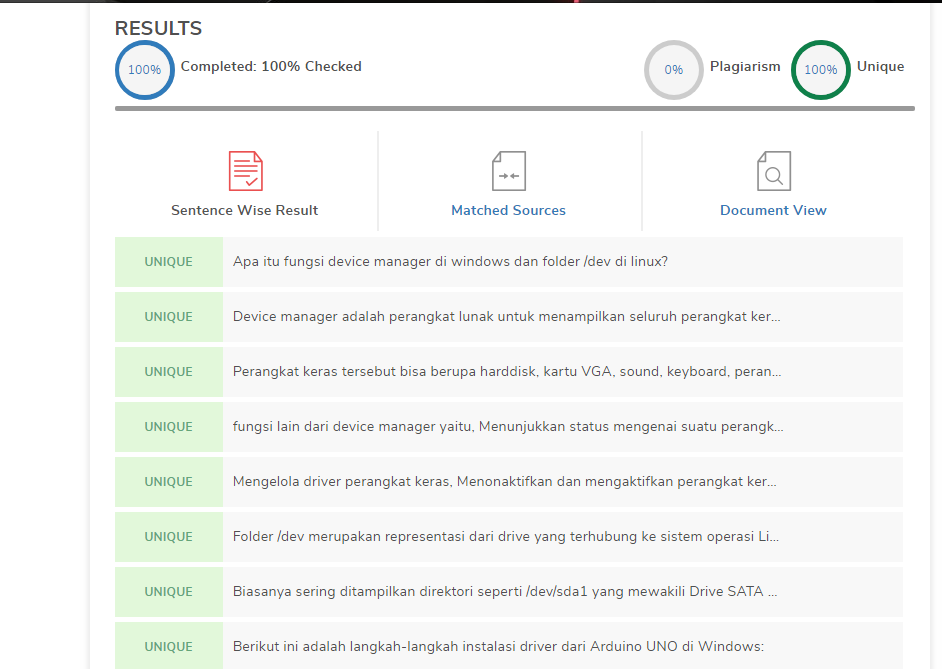
\includegraphics[width=10cm]{figures/chapter5/1174057/teori/plagiarisme.png}
		\centering
		\caption{Hasil cek plagiat}
	\end{figure}
